\documentclass[tufte-handout]{standalone}
\usepackage{mathpazo} % Sets Palatino as the main font
\usepackage{tikz}
\usetikzlibrary{3d, angles, quotes, calc, backgrounds}
\usetikzlibrary{decorations.markings,shapes.geometric, arrows, positioning}

% my colors
\definecolor{darkslategray}{rgb}{0.18, 0.31, 0.31}
\definecolor{myorange}{rgb}{0.89804, 0.55686, 0.19608}

\tikzstyle{first} = [rectangle, rounded corners, minimum width=3cm, minimum height=1cm, text centered, fill=darkslategray!20, draw=darkslategray!80!black, font=\bfseries\itshape]
\tikzstyle{second} = [rectangle, rounded corners, minimum width=3.75cm, minimum height=1cm, text centered, fill=myorange!20, draw=myorange!80!black, font=\bfseries] 

\tikzstyle{arrow} = [thick,->,>=stealth]
\tikzstyle{line} = [thick,-,>=stealth]


\begin{document}

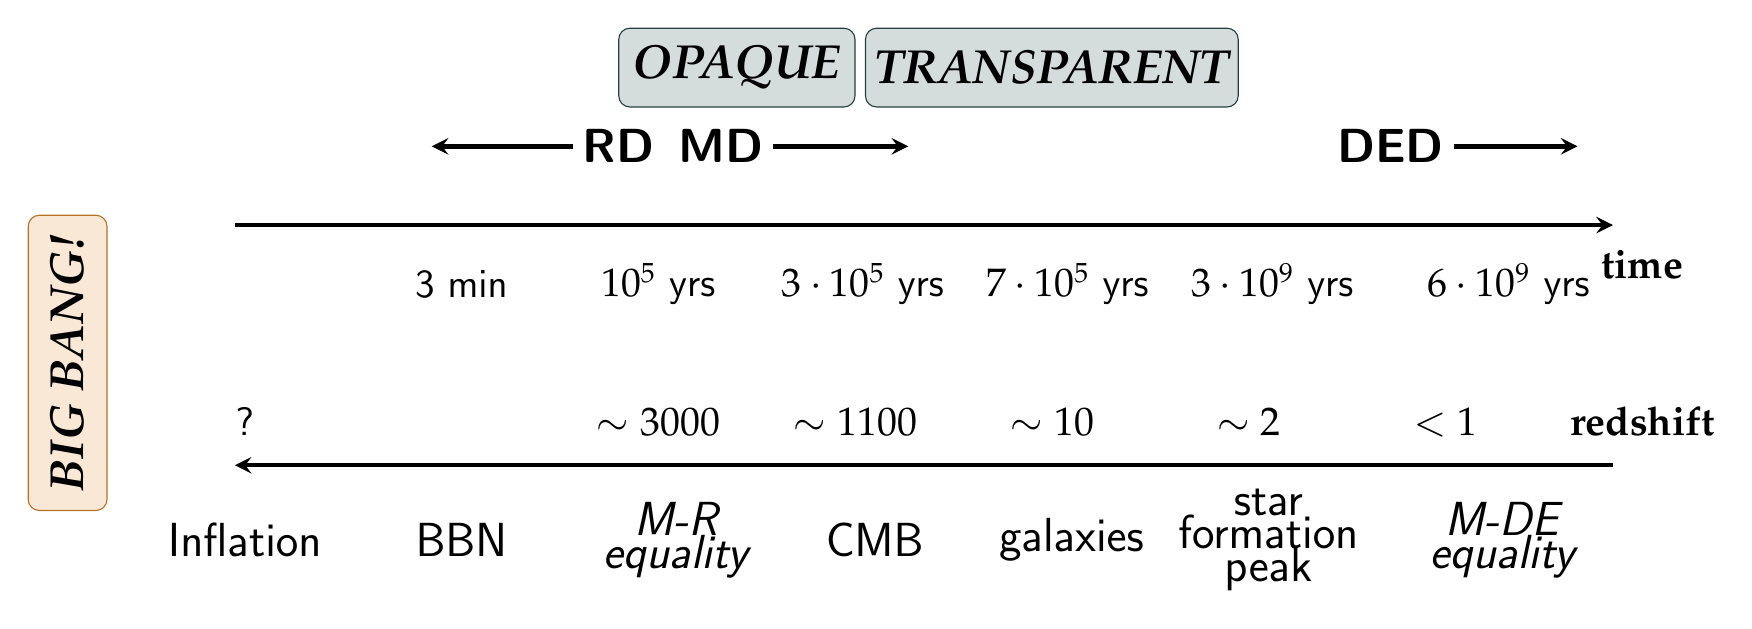
\begin{tikzpicture}[node distance=2.5cm, scale=2, every node/.style={fill=white, font=\sffamily}, align=center]


\node (plasma) [first] {\LARGE{\textbf{OPAQUE}}};
\node (light) [first, right of=plasma, xshift=1.5cm]{\LARGE{\textbf{TRANSPARENT}}};


\node (RD) [below of=plasma, yshift=1.5cm, xshift=-1.5cm] {\LARGE\textbf{RD}};
\node (arrowRD) [left of=RD] {};
\draw[arrow, ultra thick] (RD) -- (arrowRD);

\node (BBNtime) [below of=arrowRD, yshift=0.75cm, xshift=0.5cm] {\Large 3 min};

\node (MReqtime) [right of=BBNtime] {\Large $10^5$ yrs};
\node (MReqz) [below of=MReqtime, yshift=0.75cm] {\Large $\sim 3000$};
\node (inflz) [left of=MReqz, xshift=-2.75cm] {\Large ?};
\node (CMBtime) [right of=MReqtime, xshift=0.1cm] {\Large $3\cdot 10^5$ yrs};

\node (CMBz) [right of=MReqz] {\Large $\sim 1100$};

\node (galtime) [right of=CMBtime, xshift=0.1cm] {\Large $7\cdot 10^5$ yrs};

\node (galz) [right of=CMBz] {\Large $\sim 10$};

\node (startime) [right of=galtime, xshift=0.1cm] {\Large $3\cdot 10^9$ yrs};

\node (starz) [right of=galz] {\Large $\sim 2$};

\node (MDEeqtime) [right of=startime, xshift=0.5cm] {\Large $6\cdot 10^9$ yrs};

\node (MDEeqz) [right of=starz] {\Large $<1$};

\node (BBN) [below of=BBNtime, align=center, yshift=-0.75cm] {\LARGE BBN};

\node (inflation) [left of=BBN, xshift=-0.25cm] {\LARGE Inflation};

\node (MReq) [right of=BBN, xshift=0.25cm] {\LARGE\textit{M-R} \\\LARGE\textit{equality}};

\node (CMB) [right of=MReq] {\LARGE CMB};

\node (gal) [right of=CMB] {\LARGE galaxies};

\node (stars) [right of=gal] {\LARGE{star}\\\LARGE{formation}\\\LARGE{peak}};

\node (MDEeq) [right of=stars, xshift=0.5cm] {\LARGE\textit{M-DE}\\\LARGE\textit{equality}};

\node (MD) [right of=RD, yshift=0cm, xshift=-1.2cm] {\LARGE\textbf{MD}};
\node (arrowMD) [right of=MD] {};
\draw[arrow, ultra thick] (MD) -- (arrowMD);

\node (DE) [right of=MD, xshift=6cm] {\LARGE\textbf{DED}};
\node (arrowDE) [right of=DE] {};
\draw[arrow, ultra thick] (DE)--(arrowDE);

\node (BB) [second, rotate=90, below of=arrowRD, xshift=-2.75cm, yshift=7cm]  {\LARGE\textit{BIG BANG!}};

\node (anchorBBNW) [right of=BB, yshift=1.75cm, xshift=-0.5cm] {};
\node (anchorBBSW) [right of=BB, yshift=-1.3cm, xshift=-0.5cm] {};

\node (anchorBBNE) [right of=BB, yshift=1.75cm, xshift=17.25cm] {};
\node (anchorBBSE) [right of=BB, yshift=-1.3cm, xshift=17.25cm] {};

\draw[arrow, ultra thick, ->] (anchorBBNW) -- (anchorBBNE);

\node (time) [below of=anchorBBNE, yshift=2cm, xshift=0.25cm] {\Large \bf time};

\node (z) [below of=time, yshift=0.5cm, xshift=0cm] {\Large \bf redshift};

\draw[arrow, ultra thick, ->] (anchorBBSE) -- (anchorBBSW);

\end{tikzpicture}
\end{document}
